\documentclass[letterpaper,10pt,draftclsnofoot,onecolumn,titlepage]{IEEEtran}

\usepackage{graphicx}
\usepackage{amssymb}
\usepackage{amsmath}
\usepackage{amsthm}
\usepackage{alltt}
\usepackage{float}
\usepackage{color}
\usepackage{url}
\usepackage{enumitem}
\usepackage{pstricks, pst-node}
\usepackage{geometry}
\usepackage{array}
\usepackage{listings}
\usepackage{caption}
\usepackage{subcaption}
\usepackage{import}
\usepackage[draft]{pdfpages}


\geometry{margin = .75in}

\usepackage{hyperref}

\usepackage[acronym]{glossaries}

\makeglossaries

\newglossaryentry{iOS}{name={iOS}, description={A mobile operating system created and developed by Apple Inc. exclusively for Apple's hardware}}
\newglossaryentry{ModelVC}{name={Model-View-Controller}, description={A design pattern that assigns objects in an application one of three roles: model, view, or controller. Also called MVC}}
\newglossaryentry{Android}{name={Android}, description={A mobile operating system developed by Google, based on the Linux Kernel and designed primarily for touchscreen mobile devices}}
\newglossaryentry{App}{name={app}, description={A software application designed to run on mobile devices such as smartphones or tablet computers}}
\newacronym{ccb}{CCB}{Church Community Builder}
\newacronym{sdd}{SDD}{Software Design Document}
\newacronym{srs}{SRS}{Software Requirements Specification}
\newacronym{uml}{UML}{Unified Model Language}
\newacronym{mvc}{MVC}{Model-View-Controller}
\newacronym{xml}{XML}{EXtensible Markup Language}
\newacronym{ui}{UI}{User Interface}



\graphicspath{{figures/}{pictures/}{images/}{./}}


\newcommand*{\signature}[1]{%
	\par\noindent\makebox[3.5in]{\hrulefill} \hfill\makebox[3.0in]{\hrulefill}%
	\par\noindent\makebox[3.5in][l]{#1}	    \hfill\makebox[3.0in][l]{Date}%
}%

\def\name{Kevin Stine, Courtney Bonn, Maxwell Dimm}
\def\team{Calvary Chapel Corvallis}
\def\grp{Group \#62}

\hypersetup{
	colorlinks = true,
	urlcolor = black,
	linkcolor = black,
	pdfauthor = {\name},
	pdftitle = {CS463 Final Report},
	pdfsubject = {CS463 Final Report},
	pdfpagemode = UseNone
}

\begin{document}
	\title{\huge \team \\ Final Report\\ CS 463 Spring 2017}
	\author{\large \name \\ \grp}



	\maketitle

		\begin{abstract}The purpose of this project is to produce an iOS/Android application for Calvary Chapel of Corvallis that will allow members to access a plethora of information all in one localized space.
		The Church's current website does not provide an interface where current members of the church can very quickly access important information such as events, bulletins, and messages from the service.
		The desired application will be simple enough for anyone to use while providing back end access for staff to easily upload new information to the app.
		The priorities lie in maximizing the usability of the app and providing bulletin, schedule, video, and giving functionality.
		We will work with the existing Calvary Chapel web development team to create a product that is seamlessly integrated with their already existing network.
		\end{abstract}

		\clearpage
		
		\tableofcontents
		
		\clearpage

\section{Introduction}

\section{Original Requirements}

	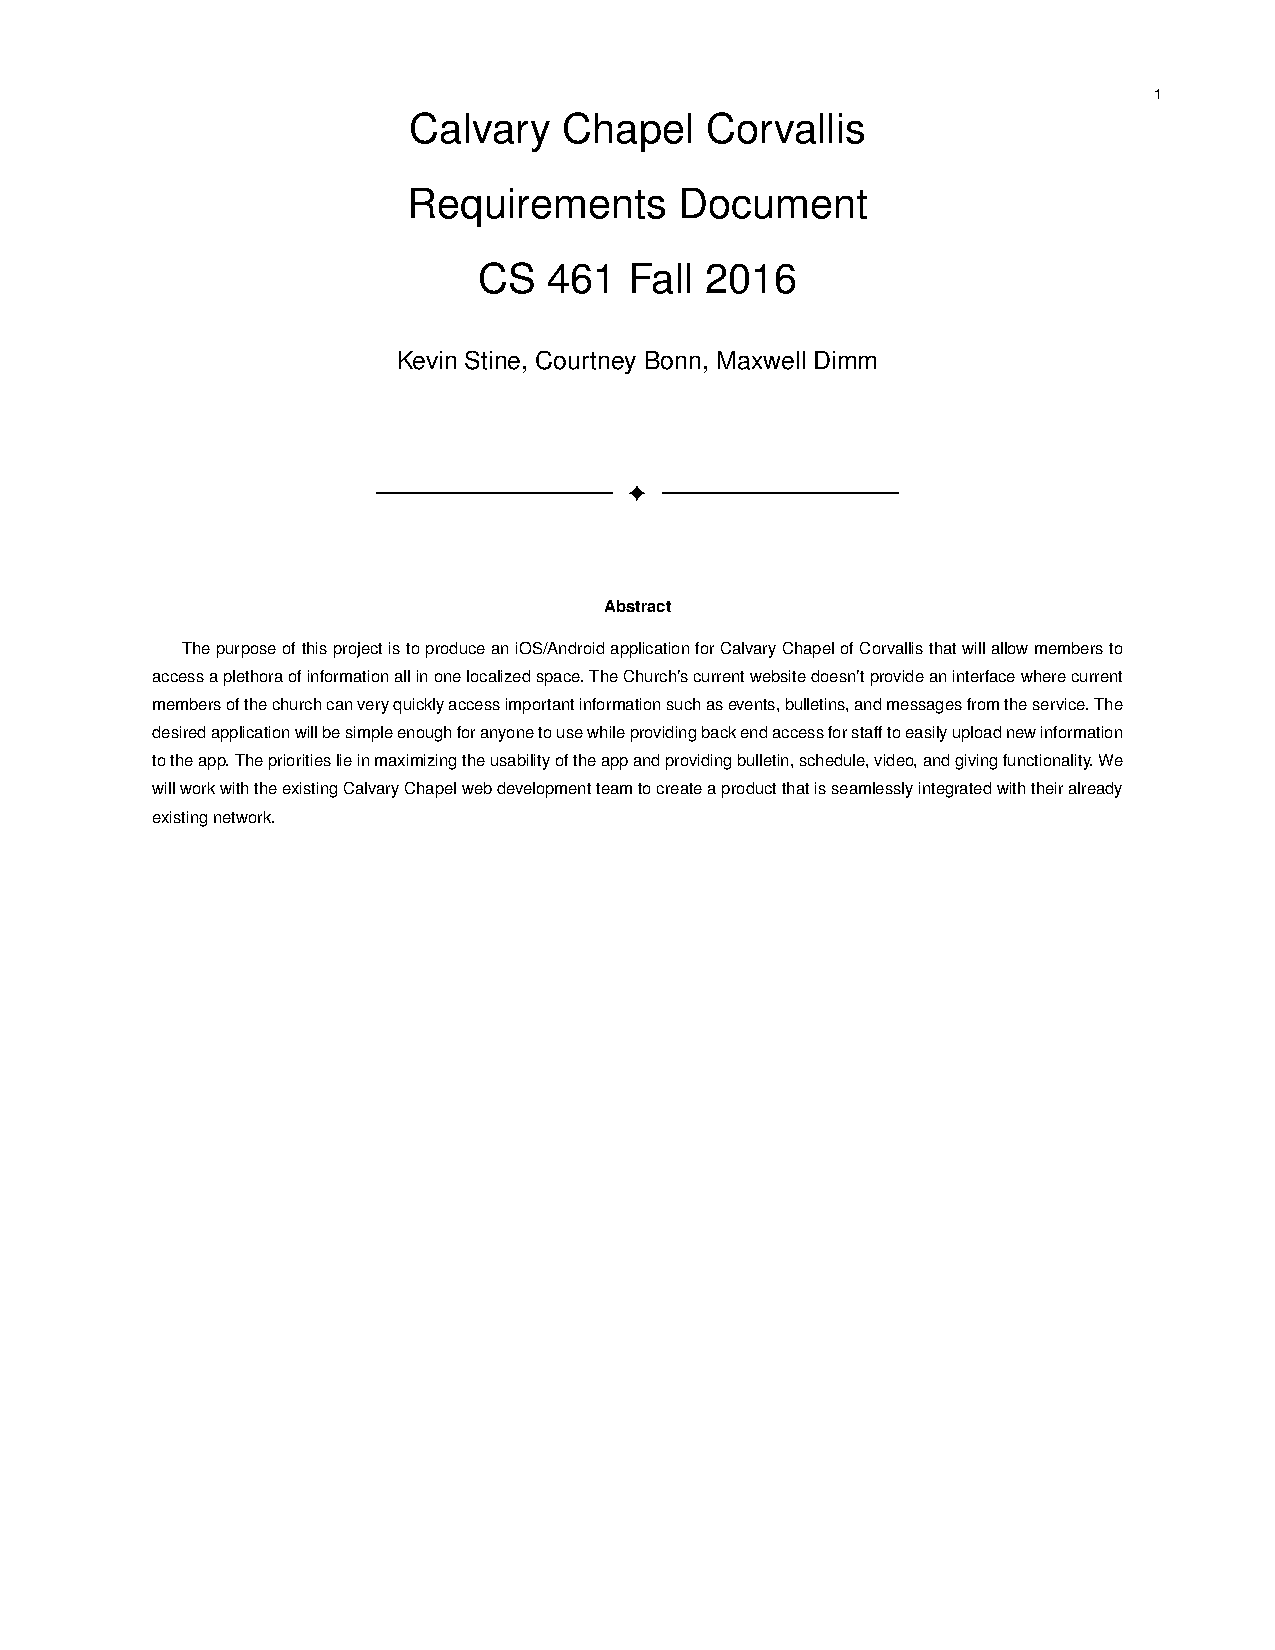
\includepdf[pages={-}]{originals/requirements.pdf}

\section{Requirement Changes}

\section{Original Design Document}

	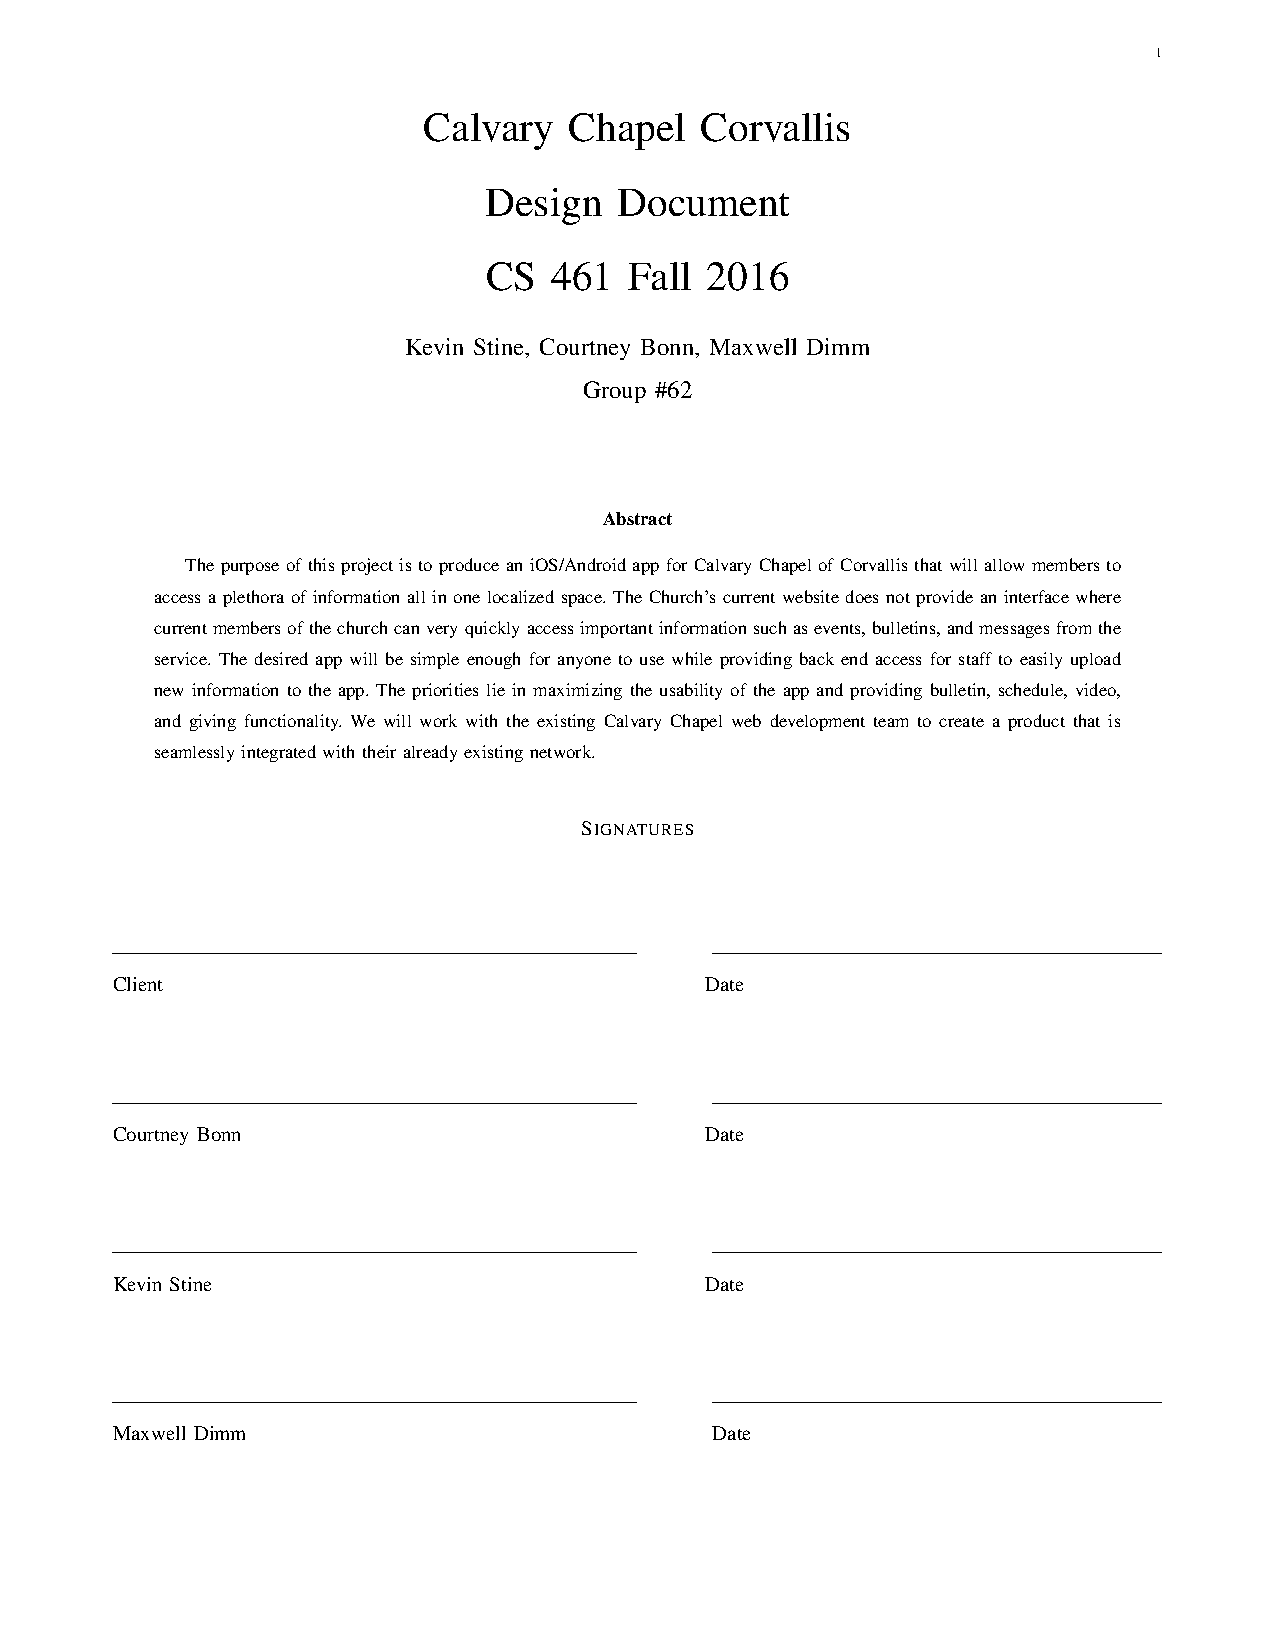
\includepdf[pages={-}]{originals/design.pdf}
	
	\subsection{Design Changes}
	
\section{Original Technology Review}

	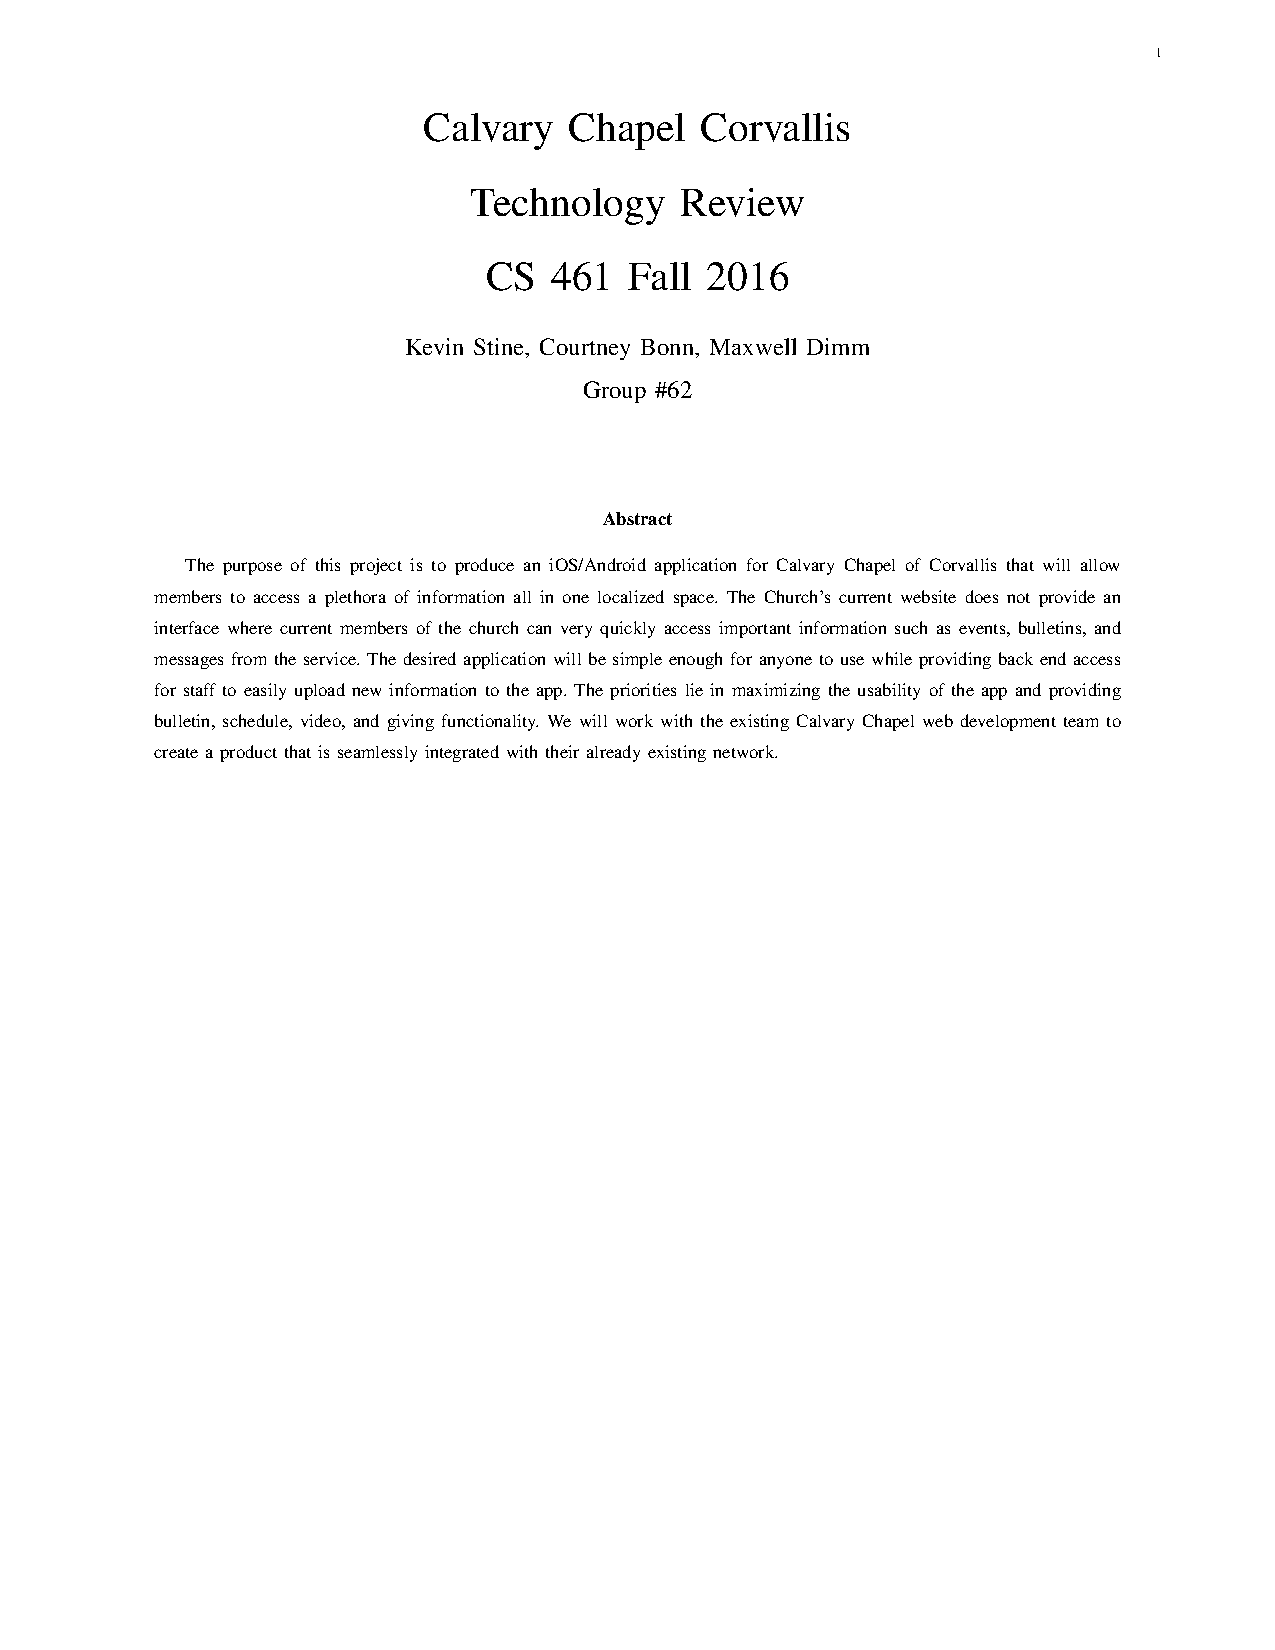
\includepdf[pages={-}]{originals/tech-review.pdf}

	\subsection{Technology Changes}
	
\section{Weekly Blog Posts}

	\subsection{Fall 2016}
	
		\subsubsection{Week 3}
		
			\paragraph{Courtney Bonn}
			This week we met with our client on Tuesday and met the rest of the staff at Calvary Church. At the meeting we talked about the basic idea of the application, as well as some bigger goals that we want to strive for. We also discussed what kind of design they were looking for. Like the functionality of the app, they are looking for a relatively simple design.

This upcoming week we are planning to meet with the church's website designer/developer. He has information about the church's management software that will assist us in integrating the calendar into the application. Personally, I plan to start doing a lot of research this upcoming week on creating iOS/Android applications.

			\paragraph{Max Dimm}
			This week we actually went to calvary church to meet with our client and her churches existing dev team. We went over what their expectations and desires were out of the project. A lot of this info can be seen on our problem statement. However the jist of it was that they wanted an easy to use app for IOS and android that gives their existing members an easy way to access weekly information. The info they wanted included on the app was things like a bulletin, schedule, videos of past messages, and the bible. There were other small things but those were the major ones.

Also this week we set up this blog and stated/finished our problem statement. For the problem statement I wrote about our solution and what we should be expected at the expo. I wrote around 300-350 words and Courtney helped me out by adding it to the tex document.
			
			\paragraph{Kevin Stine}
			This week we met with our client and hammered out the details of what our project will look like. Since we are building a mobile app based on the mobile version of their website, we met with the media and web guys to get a better idea of what they were envisioning. Since last week we were able to get all the details down and write our problem statement.

This upcoming week I plan on getting more familiar with LaTeX for future write ups, looking into mobile development for iOS and Android, and getting more familiar with the back-end software that the church utilizes.

		\subsubsection{Week 4}
		
			\paragraph{Courtney Bonn}
			We met with our client at the church and we were introduced to their website developer. This was mostly just an introduction where we gathered any additional thoughts he had on the project. He let us know that he would prefer to publish the app at the end of the year, so that way it's under his developer profile. I didn't do as much outside research on app development as I was hoping to do this week, but I am planning on doing much more this upcoming week. We also have the problem statement that we need to edit. I don't think we have too much editing to do on this paper, but I still plan on putting some more time into it. Additionally, we have the requirements document that we are going to start working on. I think the biggest goal this next week is to get a much more solid grasp onto our project, hopefully leading us into a good start on the actual project itself.

			\paragraph{Max Dimm}
			This week we met with our client again to be introduced to their lead web developer. We talked for a bit about the problem statement along with the developers ideas for the project. He was interested about how the end product would be delivered to him and how he can be included in the dev process. He informed us he has the ability to upload apps to the app store. We didnt have too much to do besides this meeting as there were no assigned papers/works alongside this. We will begin the edits on our problem statement when we are emailed our corrected first draft.
			
			\paragraph{Kevin Stine}
			This week we met with our client and got to meet their lead web developer. We picked his brain a bit to get a better idea of what he had in mind for the app, and how we could get access to some of their current resources. We got into talking about the actual deliverable and how we would be handing off the project and whether or not publishing the app would fall on us. This week I also took a look at some of the basics of developing for iOS using Swift. I started going through Apple's Swift Developer Tutorial to get a little more familiar with Xcode and Swift. Next week we'll be going through the requirements document and really hammer out the details of all the requirements we have on this project.
			
		\subsubsection{Week 5}
		
			\paragraph{Courtney Bonn}
			This week we focused on updating our problem statement and drilling down on our requirements document. We reviewed some of the requirements document with our TA to check in and make sure we were headed in the right direction. I did some research on Swift and iOS programming. I downloaded Xcode onto my Mac to start trying and learn Swift. We are at the point where we need to start thinking about whether or not we are going to build two apps (one for iOS, one for Android) or if we are going to build one app that is cross-platform. This upcoming week we need to put in some time researching what might be best for our project. We plan on meeting with our client this week to go over the requirements document and fine-tune it before turning in the final document on Friday 11/4.

			\paragraph{Max Dimm}
			This week we finished up our problem statement and began on our requirements doc. We also met our TA Vee who seemed pretty chill. We decided not to meet with our client this week because we didnt have much to deliver to her at this point, plus we had met every other week up until this point. On my end I was able to help a bit with both of the documents and deliver them on the due dates. I need to be more ontop of the documents, because by the time I get involved they most of the time have already taken form. In the future I'd like to help design or help start the documents.
			
			\paragraph{Kevin Stine}
			This week we finished up our problem statement and got that submitted based on what our client approved. I began going through a swift tutorial and have been looking into the basics for creating an application on iOS. This week we will be determining exactly what the client wants in terms of the application. Do they want two apps for both iOS and Android, or would they prefer an application for one platform in particular.
			
		\subsubsection{Week 6}
		
			\paragraph{Courtney Bonn}
			This week we focused on finishing and polishing our requirements document. We got a rough timeline for the rest of our project. We sent our requirements document to get approved by our client, who agreed with everything except for just a few small changes. Next up is beginning to research for the design document and along with that we'll begin working on the technology review. This will consist of us looking into the different technology available for us to use on our project.

			\paragraph{Max Dimm}
			So this week we were pretty much exclusively working on the requirements doc. We were able to get it done but it was a little tense getting our clients attention at one point. Once we were able to get her to work with us we could put the finishing touches on the doc and turn it in. I missed the one class of the week and my first class because I was out of town for the holiday weekend but dont plan on missing much more class. I need to start looking into app development more and finding out how I can contribute to the actual work part of our project from this point on.
			
			\paragraph{Kevin Stine}
			This week our main focus was completing the requirements document. We really took the time to verify that we documented everything that we would need to be doing for this app. This week we'll be getting started with the design document and tech review, so we'll need to really hammer out our design on the application. I plan on looking more into the different design guidelines for both iOS and Android, and coming up with some good designs and ideas for how we want to structure our application. I've been going through a Swift tutorial and will continue to explore swift in the hopes to use it for our iOS application.
			
		\subsubsection{Week 7}
		
			\paragraph{Courtney Bonn}
			We focused heavily on the technology review this week. We didn't meet with our client as we didn't have any new material to go over with her quite yet. We met up just with our group and hashed out the different parts of our system that we need to researched. Once we figured out who was going to be working on each part, we each set out to start our individual research. I took on iOS development platform, iOS user interface organization, and integrating the e-bulletins. I'm fairly confident that each technology I chose will work well with our client, as I kept in mind the requirements and exactly what the client is expecting. This next week we will start working on the design document.

			\paragraph{Max Dimm}
			This week we are starting on our tech review which is gonna be a big project. We did not meet with our client because we did not have anything worth reviewing to go over with her yet. However we did meet as a group outside of class to go over what each of us was going to work on in the tech review. We started the process of writing but most of that will likely come down to this weekend and next week early on. I was assigned to talk about cross-platform development, sermon integration, and schedule integration.
			
			\paragraph{Kevin Stine}
			This week we got working on our tech review and I spent most of the week researching and figuring out what other technologies were available for us to potentially use for our application. I focused mainly on the Android development platform, Android UI design, and integration with a giving platform. Researching and seeing what other technologies are available was really helpful to get a better idea of what options we have moving forward. Moving forward I'll be starting to get our design document setup so we can start figuring out exactly how we want to design our app.
			
		\subsubsection{Week 8}
		
			\paragraph{Courtney Bonn}
			We finished and turned in our technology review this week. The next task is to work on our design document. I think we have a good feel for what we need to do, though we haven't begun working on it quite yet. My plan is to work on my portion of the design document at least a little bit before the Thanksgiving holiday. After that we will have the progress report along with the recorded presentation to work on for finals weeks.

			\paragraph{Max Dimm}
			I got a bit of a late start on writing my part of the tech review. I spent most of the weekend and monday working on my pieces of it but was able to get my portion done in time. It took a bit longer then I expected as the amound of sections each part was fairly large. This week we will begin looking forward and running our tech review by our client. We also did not meet as we figured the whole meeting would just be reading through the 23 page doc. We decided just sending them the doc to read on their own would make more sense.
			
			\paragraph{Kevin Stine}
			This week we wrapped up our tech review and got it turned in. I spent a lot of time looking into the Android UI design that we want to use and it was good to dive deeper into the layout that we want to use in our app. Next we have the design document which will require more detail and figuring out exactly how we want to implement our application.
		
		\subsubsection{Week 9}
		
			\paragraph{Courtney Bonn}
			With Thanksgiving holiday this week, we didn't meet with our TA or work on the design document very much. I began the outline for the document and began working on the first four sections. This upcoming week will be very busy with the design document as well as hopefully meeting with the client to go over our decisions. We will also begin working on the progress report and planning how we will complete the recorded presentation.

			\paragraph{Max Dimm}
			We had a short week this week only meeting on tuesday. We wrote to our TA Vee a short bit about what we were excited about and what we were worried about. Other then that we started our design document but I was not able to contribute much at this time due to being out of town. Next week I plan on getting my share of the work done whatever that may be. We also did not meet with our client due to the holiday weekend but we will most likely meet with them the following week.
			
			\paragraph{Kevin Stine}
			This week was a short one as we had Thanksgiving. I didn't really do much for this class this week but have begun thinking about the design document. I'll be doing a lot of research into the various viewpoints that we'll want to incorporate into our application. We'll probably meet with our client next week as it'll likely be the last time before Christmas break so we can answer any questions they might have.
			
		\subsubsection{Week 10}
		
			\paragraph{Courtney Bonn}
			With this last week of the term, we really drilled down and focused on the design document. I think we underestimated the depth of this document. Because the app that we're designing is supposed to be a simple design, we didn't realize how much effort and time would go into planning the design. We did end up finishing the design document and I think we did a great job. We also met with our client for the last time this term. We made sure we were all on the same page and answered any questions the client had. I have a good idea of where this project is going and I think it's going to be successful. During the break, I plan on doing a lot more research on iOS and Android development so that way when we start implementation in the Winter I know more of what I'm doing.

			\paragraph{Max Dimm}
			We got off to a bit of a slow start on the design document but were able to finish it on time. We were not super clear on the depth that was required by some of the sections/viewpoints. We were able to meet with our client before the end of the term which was good. We were able to send her the documents we had been working on and just make sure that our visions were still in sync for the project.
			
			\paragraph{Kevin Stine}
			This week we got going on the design document. Since we are all pretty new to mobile development, we weren't entirely sure how to go about mapping out our design processes for the entire application. As we begin to learn more about mobile development I'm sure we'll be able to add more in-depth information to our design document, but we had to get as much planned out based on our current skill level. We also met with our client for the last time before break so we could make sure to get on the same page about everything moving forward. Once break begins I plan on heavily researching iOS and Android development. I'd like to have a full-functioning layout of our application for both platforms before Winter term begins so we can focus on integrating the Church's database and information into our app without worrying about the layout.
		
	\subsection{Winter 2017}
	
		\subsubsection{Week 1}
		
			\paragraph{Courtney Bonn}
			During Winter break, I didn't accomplish nearly as much as I wished I had. I ended up being very busy with work and family obligations and wasn't able to work on this project. I have started looking in to Android Studio as I am using it for another class so this will be beneficial for our project. My goal within the next week is to finish up the Swift tutorial so we can get going on our project. Kevin set up the skeleton of our iOS app and we verified we were all able to pull it from Git and run it. I've also touched base with our client. We've agreed that we don't have any reason to meet thus far and will put our first meeting off a few weeks until we have something to present.

			\paragraph{Max Dimm}
			Over the break I really only downloaded x-code and experemented with it without much real purpose. I looked up a few guides but knowledge did not really stick. The first week I spent my time downloading getkraken on my macbook and downloaded Kevins skeleton. We did not meet with our client because we didnt really have much to go over with her but we plan to do so in the next week or two I think. My goals for next week are to start looking over some of the swift guides online and start learning the language.
			
			\paragraph{Kevin Stine}
			Over break I really didn't have much of an opportunity to dive deeper into App Development besides for just looking at some of the iOS documentation. I was able to setup a pretty basic app with multiple pages like we want for our application for Calvary Chapel. This will work pretty well as a foundation for building up the other aspects of the app, however there is a lot that we'll need to do in order to get this app fully functioning in the next few months. My next steps will be to dive deeper into looking at the documentation for the various APIs that we wish to use in order to bring in the functionality for the calendar or sermons.
			
		\subsubsection{Week 2}
		
			\paragraph{Courtney Bonn}
			This week I focused heavily on learning Swift and Xcode. I wasn't able to work on it during break, so I do feel a little behind in terms of our project. We have a basic template for our iOS app that has different pages and icon images, but our next step would be to start pulling in the actual information. I've emailed our client to get some clarifying information on the Church's new website. I believe the new website is using Wordpress (from looking at the site and the Web Inspector tool via Safari) which will allow us to use Wordpress' API to bring information to the app--allowing the web development team to only have to update the site and it will in turn update the app. I'm waiting for an answer on this now and will then start looking into Wordpress API further.

			\paragraph{Max Dimm}
			This week I began the process of looking over the swift guides we found online. I dont think I'm currently where I want to be with learning the language just yet. It's starting to feel like it might be one of those things where I just need to start working on it and look up the parts as I go. I believe my next steps are to either start working on the sermons functionality or the donations. I will need to see how to go about how to implement the IOS media player in the app so we can show the messages.
			
			\paragraph{Kevin Stine}
			This week I focused more on getting familiar with iOS development and I continued to refine the basic framework of an app that I created earlier. I've mostly been adding small features and getting a feel for how everything is laid out in Xcode so that as we move forward I'll have a better grasp on the platform we're using. I will begin working on getting the events page setup with a table view that pulls from the Church's database and populates the table with the events as well as the dates.

		
		\subsubsection{Week 3}
		
			\paragraph{Courtney Bonn}

			\paragraph{Max Dimm}
			
			\paragraph{Kevin Stine}
			
		\subsubsection{Week 4}
		
			\paragraph{Courtney Bonn}

			\paragraph{Max Dimm}
			
			\paragraph{Kevin Stine}
			
		\subsubsection{Week 5}
		
			\paragraph{Courtney Bonn}

			\paragraph{Max Dimm}
			
			\paragraph{Kevin Stine}
			
		\subsubsection{Week 6}
		
			\paragraph{Courtney Bonn}

			\paragraph{Max Dimm}
			
			\paragraph{Kevin Stine}
			
		\subsubsection{Week 7}
		
			\paragraph{Courtney Bonn}

			\paragraph{Max Dimm}
			
			\paragraph{Kevin Stine}
			
		\subsubsection{Week 8}
		
			\paragraph{Courtney Bonn}

			\paragraph{Max Dimm}
			
			\paragraph{Kevin Stine}
		
		\subsubsection{Week 9}
		
			\paragraph{Courtney Bonn}

			\paragraph{Max Dimm}
			
			\paragraph{Kevin Stine}
			
		\subsubsection{Week 10}
		
			\paragraph{Courtney Bonn}

			\paragraph{Max Dimm}
			
			\paragraph{Kevin Stine}
			
	\subsection{Spring 2017}
	
		\subsubsection{Week 1}
		
			\paragraph{Courtney Bonn}

			\paragraph{Max Dimm}
			
			\paragraph{Kevin Stine}
			
		\subsubsection{Week 2}
		
			\paragraph{Courtney Bonn}

			\paragraph{Max Dimm}
			
			\paragraph{Kevin Stine}
		
		\subsubsection{Week 3}
		
			\paragraph{Courtney Bonn}

			\paragraph{Max Dimm}
			
			\paragraph{Kevin Stine}
			
		\subsubsection{Week 4}
		
			\paragraph{Courtney Bonn}

			\paragraph{Max Dimm}
			
			\paragraph{Kevin Stine}
			
		\subsubsection{Week 5}
		
			\paragraph{Courtney Bonn}

			\paragraph{Max Dimm}
			
			\paragraph{Kevin Stine}
			
		\subsubsection{Week 6}
		
			\paragraph{Courtney Bonn}

			\paragraph{Max Dimm}
			
			\paragraph{Kevin Stine}
			
		\subsubsection{Week 7}
		
			\paragraph{Courtney Bonn}

			\paragraph{Max Dimm}
			
			\paragraph{Kevin Stine}

		
\section{Final Poster}

\section{Project Documentation}

\section{Learning New Technology}

\section{Team Reflection}

	\subsection{Courtney Bonn}
	
	\subsection{Max Dimm}
	
	\subsection{Kevin Stine}
	


\end{document}
